\chapter{序論}
我々の身の回りにある物質を構成する最小単位は素粒子である。
物質の最小単位である素粒子と、素粒子の相互作用を記述した理論として標準模型が存在している。素粒子物理学において、自然界には電磁相互作用、強い相互作用、弱い相互作用、重力相互作用といった4種類の基本相互作用が存在すると考えられており、標準模型では重力相互作用以外の3種類の相互作用が記述されている。
標準模型は図\ref{fig:標準模型}に示すように、12種類のフェルミオン、4種類のゲージボソン、ヒッグス粒子の計17種類の粒子から構成されており、唯一実験的に未確認であったヒッグス粒子も2012年に発見された\cite{article:Higgs_boson}。
\begin{figure}[tb]
  \centering
  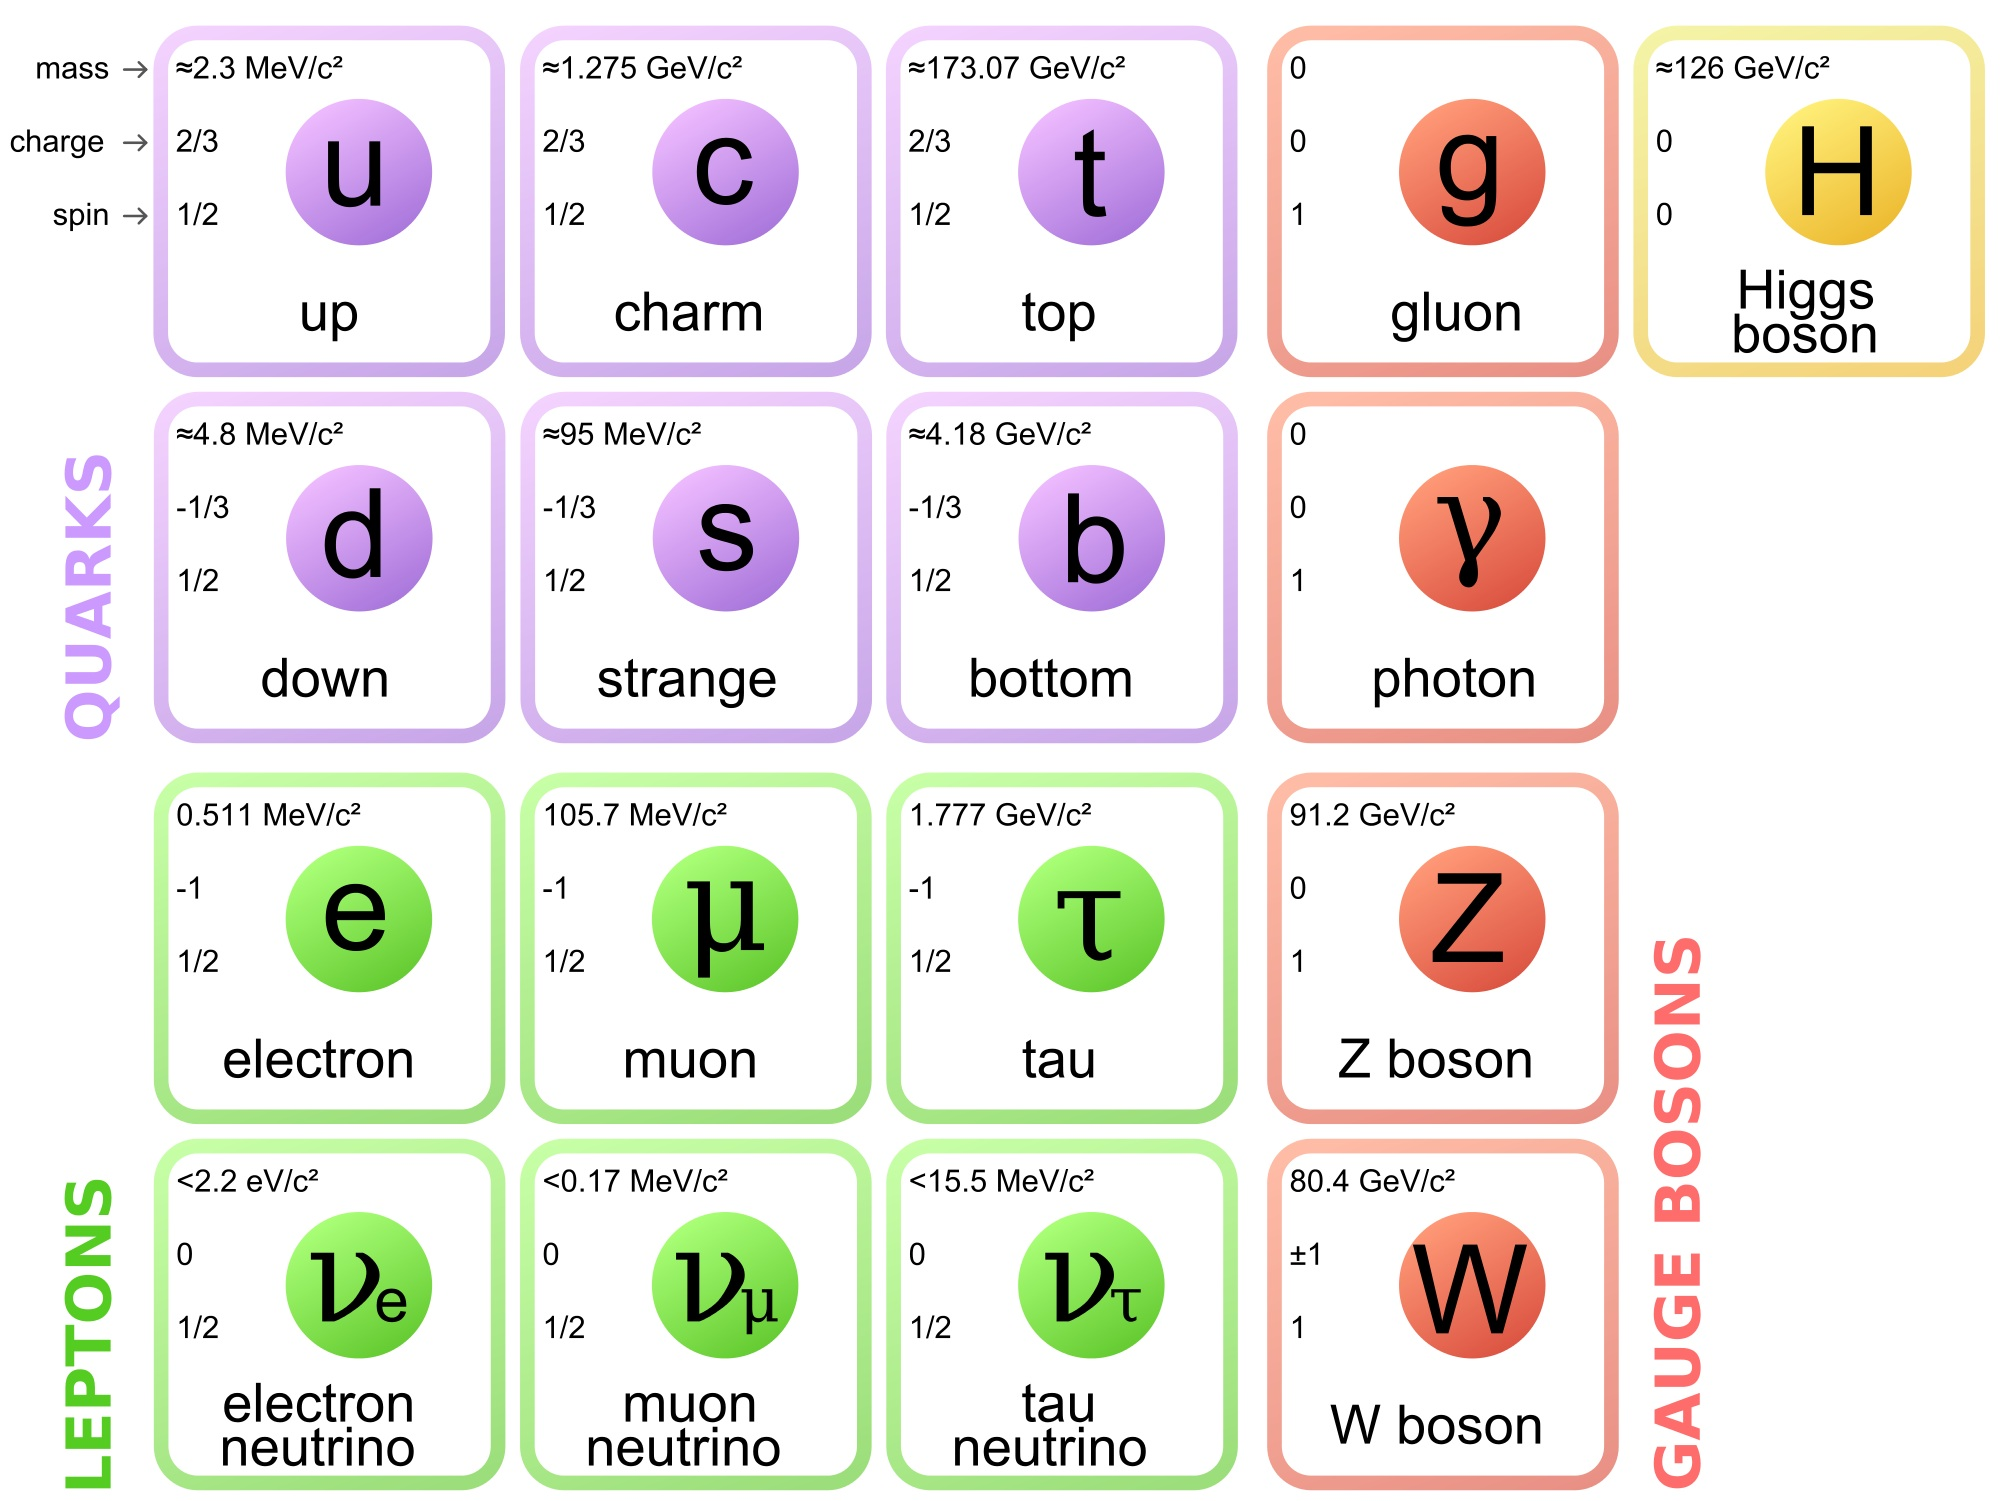
\includegraphics[clip, width=10cm]{fig/1/standardmodel.jpg}
  \caption{標準模型を構成する17種類の素粒子\cite{article:elementary_particles}。}
  \label{fig:標準模型}
\end{figure}

現在、標準模型は多くの物理事象を説明することができているが、暗黒物質の存在やヒッグス粒子の質量階層性問題などの多くの未解決問題が残されている。
この問題を解決するためには、標準模型を超える新しい物理が必要であり、この新物理を探索するためのアプローチとして世界中で様々な実験が行われている。

新物理探索の実験の一つとして、ジュネーブ郊外に位置する欧州原子核研究機構~(CERN)~\cite{article:CERN}の地下に設置された Large Hadron Collider~(LHC)~\cite{article:LHC}を用いる高エネルギーの陽子-陽子衝突実験がある。このLHCを使った衝突実験の1つであるATLAS実験~\cite{Aad:1129811}では、ATLAS検出器と呼ばれる大型汎用検出器を用いて高エネルギーの陽子-陽子衝突から粒子の測定を行い、TeVスケールまでの新粒子探索や素粒子の精密測定などの探索を行っている。

LHCではバンチと呼ばれる約$10^{11}$個の陽子の塊を単位として陽子を加速させている。LHCで行われている陽子-陽子衝突実験において、このバンチ衝突の頻度は40~MHzの高頻度のため、計算機リソースやデータ記憶容量など制限から全ての衝突事象を保存することができない。そのため、トリガーシステムと呼ばれる事象選別のアルゴリズムを用いることで、膨大な量の衝突事象から物理として興味のある事象を選別し、保存可能なデータ量まで事象数を減らしてから保存している。

ATLAS検出器では大きく分けて2段階のトリガーシステムを実装している。1段目にはハードウェアベースの高速処理が可能な初段L1トリガーがあり、測定したデータに対して一番初めにトリガー判定を行い、100~kHz以下まで事象数を落とす。2段目にはソフトウェアベースで詳細な計算が可能な後段トリガーがあり、L1トリガーで選別した事象に対して厳密なトリガー判定を行うことで、さらに数kHzまで事象数を落とす。

LHC及びATLAS検出器は2018年から2022年までの期間にアップグレードが行われ、2022年7月から第三期運転~(Run-3)が再開された。Run-3では陽子-陽子衝突の重心系エネルギーの増強や高いルミノシティでの安定した運転に伴い事象頻度がさらに増加する。したがって、限られたデータ容量の中で物理事象を最大効率で取得するために、初段トリガーにおいてもトリガーシステムの改良を行い、トリガー効率を向上させる必要がある\cite{article:phase-1}。

ミューオンは陽子-陽子衝突実験において様々な物理事象のサインとして重宝されており、トリガーシステムの中にはミューオンを用いたトリガーが実装されている。例えば、ヒッグス粒子の崩壊先である$Z$ボソンや$W$ボソンの終状態として高い運動量のミューオンが観測されやすいことや、ボトムクォークやチャームクォークが含まれる粒子の終状態には運動量が低いミューオンが含まれている。そのため、ミューオンを用いたトリガーは重要な役割を担っている。
本研究では、この初段トリガーの中でもミューオンの運動量を指針として事象選別を行う初段ミューオントリガーに着目する。

本論文ではミューオンをターゲットにして事象選別を行う初段ミューオントリガーを改良し、トリガー性能の評価を行う。第\ref{chapter2}章でLHC-ATLAS実験のの概要について述べ、第\ref{chapter3}章で初段ミューオントリガーシステムについて述べる。
第\ref{chapter4}章で本研究の主題である機械学習を用いたCoincidence Window~(CW)の作成手法の詳細について説明し、第\ref{chapter5}章で作成したCWを用いた際のトリガー性能の評価について述べた後、第\ref{chapter6}章で本研究の成果をまとめ、今後の展望について述べる。


